%Dans ce chapitre, nous étudions l’évolution d’un gaz quantique unidimensionnel après une rupture de symétrie initiale. Nous utilisons un gaz de bosons ultra-froids, confiné dans une géométrie unidimensionnelle. Ce gaz est décrit par le modèle intégrable de Lieb-Liniger. Les interactions entre atomes sont faibles et répulsives.

%Nous préparons d’abord un gaz homogène (Fig \ref{fig:BiPart.insitut}). Ensuite, nous supprimons brutalement une moitié du nuage. Cela crée une frontière nette entre deux zones : une avec des atomes , l’autre vide (Dans notre protocole la partie sans des atomes se trouve en $x<0$ et avec atomes en $x>0$) (Fig \ref{fig:BiPart.coupure1} (a),(b),(c),(d)). Cette configuration correspond à ce qu’on appelle un « quench bipartite ».


%\begin{figure}[H]
%	\centering
%	\begin{subfigure}[b]{0.3\textwidth}
%		\begin{tikzpicture}
%			\begin{scope}[shift={(2,0)}]
%				\begin{scope}[transform canvas={scale=0.6}]
					%\input{Figures/Fonc_A_code}	
			
%				\end{scope}
			
%				\draw[color = red , scale = 0.5 , draw = none  ] (-2 , -1) rectangle (5, 6) ; 	
%			\end{scope}
					
%		\end{tikzpicture}
%		\caption{}
%		\label{fig:grap.A}
%	\end{subfigure}
%	\hfill
%	\begin{subfigure}[b]{0.65\textwidth}
%		\begin{tikzpicture}

%			\begin{scope}[shift={(-11,2.7)}]
%				\begin{scope}[transform canvas={scale=0.6}]
					%% Définition des couleurs avec les codes HTML
\definecolor{colorOne}{HTML}{443E46}
\definecolor{colorTwo}{HTML}{F6DEB8}
\definecolor{colorThree}{HTML}{908CA4}
\definecolor{colorFour}{HTML}{57659E}
\definecolor{colorFive}{HTML}{C57284}
\definecolor{colorSix}{HTML}{FF5B69}

% Raccourcis pour les couleurs
\def\colorOne{colorOne}
\def\colorTwo{colorTwo}
\def\colorThree{colorThree}
\def\colorFour{colorFour}
\def\colorFive{colorFive}
\def\colorSix{colorSix}

\def\colorslide{blue!50!black}

\def\Occupation{
	\def\traitx{0.3}
	\def\traity{0.5}
	\draw[shift={(0,0)}]
		(-13.5 , 0 ) edge [thick,line width=0.8ex ]( -3.2  , 0 )
		( -3.2 - \traitx  , 0 - \traity ) edge [thick,line width=0.8ex ]( -3.2 + \traitx  , 0 + \traity  )
		( -2.8 - \traitx  , 0 - \traity ) edge [thick,line width=0.8ex ]( -2.8 + \traitx  , 0 + \traity  )
		(-2.8 , 0 ) edge [thick,line width=0.8ex ](2.8  , 0 )
		( 2.8 - \traitx  , 0 - \traity ) edge [thick,line width=0.8ex ]( 2.8 + \traitx  , 0 + \traity  )
		( 3.2 - \traitx  , 0 - \traity ) edge [thick,line width=0.8ex ]( 3.2 + \traitx  , 0 + \traity  )
		(3.2, 0 ) edge [thick,line width=0.8ex,->,>=triangle 45 , color = black ]node [pos=1.01,below  ]{\huge$\theta$}	( 13  , 0 )
	;
	\draw[shift={(0,0)}, color=\colorOne]
		(-10.5 , -1.5 ) edge [thick,line width=0.8ex , ->,>=triangle 45  ]( -10.5  , 4.5 )
	;
		
	\foreach \r in {1 , ... , 3 } {
%		\draw[
%		decoration={
%		markings,
%    	mark connection node=my node,
%    	mark=at position 0 with{\node [blue,transform shape] (my node) {\large \r};}},
%		color=gray, thick, 
%		line width=0.5ex] decorate { 
%            (-11.0, \r) -- (-10.1, \r )}
%        ;
        \draw[
			color=\colorOne,
			] 
            (-11.0, \r) edge[color=\colorThree , thick,line width=0.5ex] node [pos=-0.5 ]{\large\color{\colorFour} $\frac{\r}{\delta \theta}$ } (-10.3, \r )
        	;
	
	}
	

	
	% Graduation abcsisse 
	% Définitions des listes
% Definitions of the lists
\def\listetuple{-9/\theta_{1}, -8/\theta_{2} , -5/\theta_{3} , -2/\theta_{a-1} , 0/\theta_{a} , 1/\theta_{a+1} , 2/\theta_{a+2} ,  5/\theta_{N-4} , 7/\theta_{N-3},8/\theta_{N-1},9/\theta_{N} }
\def\listetrais{-12 , -11, -10, -9 , -8 , -7 ,  -6 , -5, -4.5,-4, -2 , -1, 0 , 0.5, 1, 2, 4 , 5 ,  6 , 7 , 8 ,8.5, 9 ,  10 , 11, 12 }

% Loop over listetrais
\foreach \r in \listetrais {
    % Initialize found variable to zero
    % Initialize found variable to zero
    %\pgfmathsetmacro\found{0}
    \global\def\found{0}
    \xdef\nomtheta{}
    
    % Check if \r is in listetuple
    \foreach \x/\y in \listetuple { 
        \ifdim \r pt=\x pt % If \r matches any \x in listetuple
            \global\def\found{1} ;
            \xdef\nomtheta{\y} % Set \nomtheta to the corresponding \y
            %\pgfmathsetmacro\found{1} % Set found to 1            
            %\global\pgfmathsetmacro\found{1}
        \fi
    }
    
    %\node [circle, draw, red] (A) at (\r, 2) {\found , $\nomtheta$};
    
    % Draw the line and display \nomtheta if found
    \ifnum\found=1
        \draw[color=\colorOne, thick, line width=0.5ex] 
            (\r, -0.3) -- (\r, 0.3) node[red , pos=-0.5] {\large $\nomtheta$};
         \filldraw[line width=0.5ex, color=\colorSix, outer color=\colorSix, inner color=\colorSix] 
            (\r, 0) circle (4pt);
    \else 
        % Draw without \nomtheta and add a blue circle if not found
        \draw[color=\colorOne, thick, line width=0.5ex] 
            (\r, -0.3) -- (\r, 0.3);
        \filldraw[line width=0.5ex, color=\colorSix, outer color=\colorTwo, inner color=\colorTwo] 
            (\r, 0) circle (4pt); 
    \fi
}

\def\listetrais{-9.5/\theta_{i-1}/2/3, -6.5/\theta_{i}/1/4  ,   -1.5/\theta_{j}/2/4 , 1.5/\theta_{j+1}/-1/3 , 3.5/\theta_{\ell-1}/1/3 , 6.5/\theta_{\ell}/3/4 , 9.5/\theta(\theta_{\ell+1})/-1/3 };



\foreach \r/\nomx/\y/\ys in \listetrais {
	\draw[
		decoration={
		markings,
    	mark connection node=my node,
    	mark=at position .5 with{\node [blue,transform shape] (my node) {\large \color{\colorFour} $\nomx$};}},
		color=\colorThree , thick, 
		line width=0.5ex] decorate { 
            (\r, 0.12) -- (\r, -1.2)}
        ;
     
     \ifdim \y pt > -1 pt 
     	\draw[
			decoration={
			markings,
    		mark connection node=my node,
    		mark=at position .5 with{\node [blue,transform shape] (my node) {\large \color{\colorFour} $\pi^d(\nomx) $};}},
			color=\colorThree, thick, 
			line width=0.5ex] decorate { 
            (\r, \y) -- (\r +3, \y)}
        ;
        \draw[
			decoration={
			markings,
    		mark connection node=my node,
    		mark=at position .5 with{\node [blue,transform shape] (my node) {\large \color{\colorFive} $\pi_s^d(\nomx) $};}},
			color=\colorFive, thick, 
			line width=0.5ex] decorate { 
            (\r, \ys) -- (\r +3, \ys)}
        ;
     \fi 
     \ifdim \r pt= -1.5 pt
     	\draw[
     		decoration={
			markings,
    		mark connection node=my node,
    		mark=at position .5 with{\node [blue,transform shape] (my node) {\large \color{\colorFour}  $\delta \theta $};},
    		%mark=at position 0.1  with {\arrow[blue, line width=0.5ex]{<}},
    		%mark=at position 1  with {\arrow[blue, line width=0.5ex]{>}}
    		},
        	color=\colorThree,
        	thick,
        	line width=0.5ex,
        	%arrows={Computer Modern Rightarrow[line cap=round]-Computer Modern Rightarrow[line cap=round]}
   			](\r, -1.2) edge[arrows={Computer Modern Rightarrow[line cap=round]-}] (\r + 0.4, -1.2)decorate {
    		(\r, -1.2) -- (\r + 3, -1.2)}(\r + 2, -1.2) edge[arrows={-Computer Modern Rightarrow[line cap=round]}] (\r + 3, -1.2)
    		;
    \fi
			
	
}


			
}


\begin{scope}
	%\draw[help lines , width=1.5ex] (-8,-3) grid (8,3);\draw[help lines ,width=0.5ex , opacity = 0.5] (-3,-3) grid[step=0.1] (3,3));
	
	%\draw[help lines] 
	%	(-3,-3) edge[width=1.5ex] grid (3,3)	
	%	(-3,-3) edge[width=0.5ex , opacity = 0.5] grid (3,3)	
	%;
	\begin{scope}[shift={(0,1)},rotate=0,opacity=1,color=black]
		\Occupation	
		
		%\node[anchor=east, font=\bfseries] at (-11, 0) {\color{red}\large (T = 0 )} ;	
	\end{scope}
	
	
	
	
	\begin{scope}[shift={(-10.5,7)},rotate=0,opacity=1,color=black]
	
	\begin{scope}[shift={(-0,0)},rotate=0,opacity=1,color=black]
	
		\draw[shift={(0,0)} ,line width=1ex,rounded corners = 1ex,color=\colorOne , opacity =1 ,fill=\colorOne!00 , pattern={north east lines} , pattern color=\colorOne!00 ]
			(0 , -1 ) rectangle (5,1)
		;
		

		\begin{scope}[shift={(0.5,0.5)}]
			\draw[color=\colorOne, thick, line width=0.5ex] 
            (0, -0.3) -- (0, 0.3) ;
            \filldraw[line width=0.5ex, color=\colorSix, outer color=\colorSix, inner color=\colorSix] 
            (0, 0) circle (4pt);
            
            \node[anchor=west, font=\bfseries] at (0.2, 0) {\color{\colorSix}\large : quasi-particule};
		\end{scope}
		
		\begin{scope}[shift={(0.5,-0.5)}]
			\draw[color=\colorOne, thick, line width=0.5ex] 
            (0, -0.3) -- (0, 0.3) ;
            \filldraw[line width=0.5ex, color=\colorSix, outer color=\colorTwo, inner color=\colorTwo] 
            (0, 0) circle (4pt);
            
            \node[anchor=west, font=\bfseries] at (0.2, 0) {\color{\colorSix}\large : hole};
		\end{scope}

	\end{scope}
	
	\begin{scope}[shift={(6,0)},rotate=0,opacity=1,color=black]	
		
		\draw[shift={(0,0)} ,line width=1ex,rounded corners = 1ex,color=\colorOne , opacity =1 ,fill=\colorOne!00 , pattern={north east lines} , pattern color=\colorOne!00 ]
			(0 , -1 ) rectangle (7.5,1)
		;
		
		\node[anchor=west] at (0.5, 0.5) {\color{\colorFour}\large $\pi^d$ };\node[anchor=west, font=\bfseries] at (0.9, 0.5) {\color{\colorFour}\large : quasi-particule distribution};
		
		\node[anchor=west] at (0.5, -0.5) {\color{\colorFour}\large $\pi_h^d$ };\node[anchor=west, font=\bfseries] at (0.9, -0.5) {\color{\colorFour}\large  : hole distribution};
		
	\end{scope}
	
	\begin{scope}[shift={(14.5,0)},rotate=0,opacity=1,color=black]	
		
		\draw[shift={(0,0)} ,line width=1ex,rounded corners = 1ex,color=\colorOne , opacity =1 ,fill=\colorOne!00 , pattern={north east lines} , pattern color=\colorOne!00 ]
			(0 , -0.5 ) rectangle (7.0,0.5)
		;
		
		\node[anchor=west] at (0.5, 0) {\color{\colorFour}\large ${\color{\colorFive}\pi_s^d} = \pi^d + \pi_h^d $ };\node[anchor=west, font=\bfseries] at (2.9, 0) {\color{\colorFour}\large {\color{\colorFive} : density of states}};
		
	\end{scope}
	
	
	\end{scope}


		
	
\end{scope}

	
			
%				\end{scope}
%				\begin{scope}[scale=1]
%					\draw[color = red , scale = 1 , draw = none  ] (-1 , -1) rectangle (5, 5) ; 
%				\end{scope}	
%			\end{scope}
			
%		\end{tikzpicture}
%		\caption{}
%		\label{fig.fluctu.A}
%	\end{subfigure}
%	\caption{}
%	\label{fig:diag_fig}
%\end{figure}


%Le gaz évolue ensuite selon la dynamique de son Hamiltonien. Nous observons le déplacement de la frontière au cours du temps. Pour cela, nous mesurons le profil de densité atomique à différents temps d’évolution.

%Nous voyons que la frontière se propage de manière balistique. La largeur du profil de densité augmente de façon linéaire avec le temps. Ce comportement est prédit par la théorie de l’hydrodynamique généralisée (GHD). Cette théorie décrit comment les propriétés locales d’un système intégrable évoluent dans le temps (Fig \ref{fig:BiPart.coupure1} (e),(f),(g)). %Elle repose sur une distribution appelée « distribution de rapidité ». Cette fonction décrit la répartition des quasi-particules dans le système.

%Dans notre cas, GHD prévoit un profil de densité particulier si le gaz initial est à température nulle. Les données expérimentales sont proches de cette prédiction, mais avec de légers écarts. Ces écarts peuvent venir de la température non nulle du gaz ou d’autres imperfections expérimentales.

%Nous montrons que le profil de densité contient beaucoup d’informations. En théorie, on peut retrouver la distribution de rapidité initiale à partir du profil de frontière. Cela permettrait d’avoir une méthode d’analyse très puissante, comme une sorte de « thermomètre généralisé ». %Cependant, cette méthode est sensible au bruit dans les données, surtout dans les parties du profil où la densité est très faible. Pour contourner cela, nous utilisons un modèle simple avec trois paramètres pour approximer la distribution de rapidité. Ce modèle donne de bons résultats et reste plus robuste.

%Enfin, nous utilisons une nouvelle méthode expérimentale pour mesurer la distribution de rapidité localement (Part {??}) , à l’intérieur du profil. Nous observons une asymétrie, comme prévu par la théorie. D’un côté, la distribution est lisse et large ; de l’autre, elle est plus abrupte, comme pour un état fondamental. Cette observation confirme le comportement prédictif de la GHD, bien que la résolution spatiale limite la finesse des détails que nous pouvons observer.


%Parmi les systèmes à N corps, les modèles intégrables occupent une place particulière, notamment dans le contexte des dynamiques hors d’équilibre et de la thermalisation généralisée. Contrairement aux systèmes génériques, ces modèles présentent une infinité de constantes du mouvement, empêchant la thermalisation au sens habituel. Cela conduit à l’émergence d’une thermalisation généralisée, décrite non par l’ensemble canonique, mais par une ensemble à entropie maximale sous contraintes — souvent formalisé par l’Ensemble de Gibbs Général (GGE) \index{Ensemble Thermodynamique Général (GGE)}\index[pers]{Ensemble Thermodynamique Général (GGE), Ensemble de Gibbs Général (GGE)}.

%Un exemple pédagogique pour appréhender cette dynamique non triviale est fourni par l’expérience du pendule de Newton : des chocs élastiques entre sphères de masses égales illustrent parfaitement l’absence de thermalisation, l'énergie cinétique se propageant de manière cohérente entre les particules. Cette dynamique régulière, bien que classique, annonce les comportements typiques des systèmes intégrables quantiques où les excitations se déplacent sans diffusion.

%Dans ce cadre, le problème de Riemann en hydrodynamique — c’est-à-dire l'évolution d’un système à partir de deux états homogènes initiaux juxtaposés — fournit un test fondamental de compréhension des équations d’évolution des systèmes intégrables. Longtemps restée partiellement ouverte, la résolution complète de ce problème dans les modèles intégrables quantiques a été obtenue grâce à la formulation de la Théorie Hydrodynamique Généralisée (GHD).

%La GHD a été introduite dans [60] pour des théories des champs intégrables (comme le modèle de Sinh-Gordon ou le modèle de Lieb-Liniger décrivant un gaz de bosons 1D en interaction), et dans [59] pour les chaînes quantiques, notamment la chaîne XXZ anisotrope de Heisenberg. Ces travaux ont permis de résoudre analytiquement le problème de Riemann dans des systèmes quantiques fortement corrélés.

%Depuis, des solutions analytiques ont été obtenues pour des cas spécifiques. En particulier, une solution exacte du problème de Riemann pour la chaîne XXZ a été trouvée pour un état initial particulier [179]. Par ailleurs, une solution plus générale a été obtenue pour un gaz 1D de sphères dures, mettant en lumière l’efficacité de la GHD à capturer les phénomènes de propagation balistique et de relaxation généralisée dans un cadre quantique.

%%%%%


%Dans ce chapitre, nous étudions la dynamique hors équilibre d’un gaz quantique unidimensionnel de bosons faiblement interactifs, préparé dans un état initial présentant une rupture abrupte de symétrie. Le système est décrit par le modèle intégrable de Lieb-Liniger, et sa dynamique unitaire est analysée dans le cadre de l’hydrodynamique généralisée (GHD), un formalisme théorique développé récemment pour capturer l’évolution spatio-temporelle des observables locales dans les systèmes quantiques intégrables.

%Le protocole expérimental consiste en un "quench bipartite" : le gaz initial, homogène et à densité constante, est brutalement tronqué, de sorte que la moitié gauche du système ($x<0$) est vidée, tandis que la moitié droite ($x>0$) reste occupée (Fig.~\ref{fig:BiPart.coupure1}). Cette configuration induit une discontinuité initiale dans le facteur d’occupation $\nu(x,\theta)$, menant à une situation analogue au problème de Riemann dans les systèmes à un nombre infini de lois de conservation. Ce type de dynamique, souvent qualifié de domain wall dynamics, a été étudié en détail dans la thèse de Léa Dubois \cite{DuboisThese}, où une première analyse expérimentale de ce protocole a été réalisée.

%Dans ce travail, nous approfondissons cette étude en mettant l’accent sur la modélisation théorique fine à l’aide des outils de la GHD. Plus précisément, nous montrons que la propagation balistique observée de la discontinuité est bien décrite par la solution GHD du problème de Riemann, à température nulle comme finie. Nous analysons quantitativement les profils de densité mesurés expérimentalement et discutons en détail les écarts observés avec les prédictions théoriques idéales, en lien avec les effets thermiques et les imperfections instrumentales.

%Un point central de notre étude consiste à exploiter les solutions GHD pour reconstruire la distribution de rapidités initiale à partir du profil de densité mesuré dans la région de transition. Cette approche, que l’on peut interpréter comme une forme de thermométrie généralisée, constitue une méthode puissante pour sonder les états locaux du gaz. Nous mettons également en œuvre une nouvelle méthode expérimentale permettant de mesurer localement le facteur d’occupation $\nu(x,\theta)$ dans la région de déformation, mettant en évidence une forte asymétrie entre les deux côtés de la discontinuité, signature de la nature hors équilibre du système.


%%%%
%Dans ce chapitre, nous étudions la dynamique hors équilibre d’un gaz quantique unidimensionnel suite à une rupture initiale de symétrie. Le système étudié est un gaz de bosons ultra-froids confiné dans une géométrie unidimensionnelle, dont la dynamique est décrite par le modèle intégrable de Lieb-Liniger. Les interactions interatomiques sont faibles et de nature répulsive, ce qui permet d’explorer un régime faiblement corrélé tout en conservant des effets quantiques collectifs non triviaux.\\

%La préparation initiale consiste en un gaz homogène à profil de densité uniforme (Fig.~\ref{fig:BiPart.insitut}). Une opération de coupe abrupte est ensuite réalisée, supprimant spatialement la moitié gauche du nuage atomique. Il en résulte une condition initiale présentant une discontinuité marquée : la région $x<0$ est vide, tandis que des atomes occupent la région $x>0$ (Fig.~\ref{fig:BiPart.coupure1} (a)-(d)). Cette configuration correspond à un quench bipartite, c’est-à-dire une mise hors équilibre induite par une discontinuité initiale dans la densité.


%Après la préparation initiale, le gaz évolue selon la dynamique unitaire régie par son Hamiltonien. Pour suivre cette évolution, nous mesurons le profil de densité atomique à différents temps, ce qui permet de visualiser la propagation de la discontinuité initiale.

%Nous observons que la frontière entre les régions occupée et vide se propage de manière balistique : la largeur du profil de densité croît linéairement avec le temps. Ce comportement est en accord avec les prédictions de la théorie de l’hydrodynamique généralisée (GHD), qui fournit une description efficace de l’évolution spatio-temporelle des observables locales dans les systèmes intégrables (Fig.~\ref{fig:BiPart.coupure1} (e)-(g)).\\



%Dans notre configuration, la théorie de l’hydrodynamique généralisée (GHD) prédit un profil de densité caractéristique dans le cas d’un gaz initial à température nulle. Les mesures expérimentales obtenues sont globalement en accord avec cette prédiction, bien qu’on observe de légers écarts. Ces déviations peuvent être attribuées à une température initiale non nulle, ainsi qu’à d’éventuelles imperfections expérimentales.

%Nous montrons que le profil de densité contient une richesse d’information sur l’état initial du système. En particulier, la théorie suggère qu’il est, en principe, possible de reconstruire la distribution de rapidité initiale à partir du profil mesuré au niveau de la frontière. Cela ouvre la voie à une méthode d’analyse puissante, que l’on peut interpréter comme une forme de thermomètre généralisé dans le cadre de la GHD.\\

%Enfin, nous mettons en œuvre une nouvelle méthode expérimentale permettant de mesurer localement la distribution de rapidité au sein du profil de densité (voir Partie {??}). Nous observons une asymétrie marquée dans la forme de cette distribution : d’un côté, elle est large et lisse, tandis que de l’autre, elle présente une coupure abrupte, caractéristique d’un état proche du fondamental. Cette observation est en accord avec les prédictions théoriques de la GHD, bien que la résolution spatiale de notre dispositif limite la précision des détails accessibles.
\begin{figure}[!htb]
	\centering
	\includegraphics[width=0.5\textwidth , page = 4 ]{Shema.pdf}	
	%\caption{a) Facteur d'occupation initial $\nu(x, \theta) = \nu_0(\theta)$ correspondant à l'équilibre thermique à la température $T = 560~\mathrm{nK}$, pour une densité spatiale linéique $n_0 = 56~\mu\mathrm{m}^{-1}$, soit une potentielle chimique $\mu = 65~\mathrm{nK}$.  
%(b) Densité spatiale linéique $n(x) = \int \rho_{[\nu]}(x, \theta)\, d\theta \equiv n_0 = 56~\mu\mathrm{m}^{-1}$.  
%(c) Facteur d'occupation initial $\nu_0(\theta)$ correspondant au cas présenté en a).}
	\caption{a) Facteur d’occupation initial $\nu(x, \theta) = \nu_0(\theta)$ correspondant à un état d’équilibre thermique à la température $T = 560~\mathrm{nK}$, pour une densité linéique homogène $n_0 = 56~\mu\mathrm{m}^{-1}$. Ces paramètres correspondent à une potentielle chimique $\mu = 65~\mathrm{nK}$.
b) Densité spatiale linéique $n(x) = \int \rho_{[\nu]}(x, \theta), d\theta$, constante et égale à $n_0 = 56~\mu\mathrm{m}^{-1}$.
c) Facteur d’occupation $\nu_0(\theta)$ correspondant à la distribution thermique illustrée en a).}
	\label{fig:BiPart.insitut}
\end{figure}


Parmi les systèmes à N corps, les modèles intégrables occupent une place particulière, notamment dans le contexte des dynamiques hors d’équilibre et de la thermalisation généralisée. Contrairement aux systèmes génériques, ces modèles présentent une infinité de constantes du mouvement, empêchant la thermalisation au sens usuel. Cette contrainte conduit à l’émergence d’une thermalisation généralisée, décrite non par l’ensemble canonique, mais par un ensemble à entropie maximale sous contraintes, souvent formalisé par l’Ensemble de Gibbs Général (GGE) \index{Ensemble Thermodynamique Général (GGE)}\index[pers]{Ensemble Thermodynamique Général (GGE), Ensemble de Gibbs Général (GGE)}.

Un exemple classique pour illustrer la dynamique non diffusante typique des systèmes intégrables est celui du pendule de Newton, où des chocs élastiques entre sphères de masses égales propagent l’énergie cinétique sans dissipation. Bien que ce système soit classique, il incarne le comportement régulier que l’on retrouve dans les systèmes intégrables quantiques, où les excitations se déplacent sans diffusion.

Dans ce cadre, le problème de Riemann en hydrodynamique — c’est-à-dire l’évolution d’un système à partir de deux états homogènes juxtaposés — constitue un test fondamental de compréhension des équations d’évolution dans les systèmes intégrables. Sa résolution complète, longtemps restée partiellement ouverte, a été rendue possible par l’avènement de la Théorie Hydrodynamique Généralisée (GHD). Introduite dans le contexte des théories des champs intégrables (modèle de Sinh-Gordon, modèle de Lieb-Liniger) [??] et des chaînes quantiques (chaîne XXZ de Heisenberg) [??], la GHD a permis une avancée analytique majeure pour la description des dynamiques hors équilibre dans ces systèmes.

Depuis, plusieurs solutions analytiques du problème de Riemann ont été obtenues. En particulier, une solution exacte pour un état initial particulier dans la chaîne XXZ [??], ainsi qu’une solution plus générale pour un gaz 1D de sphères dures, ont confirmé l’efficacité de la GHD pour décrire les processus de propagation balistique et de relaxation généralisée.

Dans ce contexte, nous étudions la dynamique hors équilibre d’un gaz quantique unidimensionnel de bosons faiblement interactifs, confinés dans une géométrie 1D. Le système est décrit par le modèle intégrable de Lieb-Liniger, avec des interactions faibles et répulsives permettant l’émergence d’effets quantiques collectifs tout en restant dans un régime faiblement corrélé.

La préparation initiale consiste à créer un gaz homogène à profil de densité constant (Fig.\ref{fig:BiPart.insitut}), à température contrôlée. Une opération de coupe abrupte est ensuite réalisée : la moitié gauche du système ($x<0$) est vidée, tandis que la moitié droite ($x>0$) reste occupée (Fig.\ref{fig:BiPart.coupure1}). Ce protocole, dit quench bipartite, engendre une discontinuité initiale dans la densité atomique, analogue au problème de Riemann pour un système doté d’un nombre infini de lois de conservation. Ce type de dynamique, qualifiée de domain wall dynamics, a été étudié dans la thèse de Léa Dubois \cite{DuboisThese}, qui a permis une première analyse expérimentale de ce protocole.

Nous poursuivons et approfondissons cette étude, en analysant la dynamique unitaire du gaz à l’aide des outils de la GHD. Nous montrons que la propagation balistique de la discontinuité observée expérimentalement est bien capturée par la solution GHD du problème de Riemann, à température nulle comme finie. Le profil de densité mesuré à différents temps révèle une frontière qui se propage de manière linéaire, en bon accord avec les prédictions de la GHD (Fig.~\ref{fig:BiPart.coupure1} (e)-(g)). Des écarts résiduels sont néanmoins observés, que nous attribuons à des effets thermiques et à des imperfections instrumentales.

Un aspect central de notre approche repose sur l’exploitation des solutions GHD pour reconstruire la distribution initiale de rapidités à partir des profils de densité mesurés dans la région de transition. Cette démarche constitue une forme de thermométrie généralisée et fournit un outil puissant pour sonder les états locaux du gaz.

Enfin, nous développons une méthode expérimentale inédite permettant de mesurer localement le facteur d’occupation $\nu(x, \theta)$ dans la région de déformation. Nous observons une forte asymétrie de cette distribution : large et lisse du côté initialement occupé, coupée et abrupte du côté initialement vide, révélant ainsi la nature fondamentalement hors équilibre du système. Cette observation est en bon accord avec les prédictions théoriques de la GHD, même si la résolution spatiale limite la finesse des détails observables.

